% =====================================================================
%  monoT5 Mean-Diff Direction Analysis + Intervention — Full Experiment Report
%  Compile with:  pdflatex mean_diff_intervention_report.tex  (run twice)
%  Figure paths are relative to this file (outputs/...), so compile
%  from the 02_monot5_mean_diff_intervention/ directory.
% =====================================================================
\documentclass[11pt]{article}

\usepackage[margin=1in]{geometry}
\usepackage{amsmath, amssymb}
\usepackage{graphicx}
\usepackage{booktabs}
\usepackage{longtable}
\usepackage{array}
\usepackage{float}
\usepackage{xcolor}
\usepackage{caption}
\usepackage{subcaption}
\usepackage{enumitem}
\usepackage{listings}
\usepackage[hidelinks]{hyperref}

\definecolor{codegray}{gray}{0.95}
\lstset{
  basicstyle=\ttfamily\footnotesize,
  backgroundcolor=\color{codegray},
  breaklines=true,
  frame=single,
  columns=fullflexible,
  keepspaces=true,
}

\newcommand{\score}{\operatorname{score}}
\newcommand{\dirvec}{\ensuremath{\vec{d}}}
\newcommand{\dtc}{\ensuremath{\Delta_{\text{control}}}}
\newcommand{\dta}{\ensuremath{\Delta_{\text{attack}}}}

\title{\textbf{Mean-Diff Direction Analysis and Intervention \\[2pt]
in monoT5's Attention Heads} \\[6pt]
\large A Linear-Steering Defense and Sufficiency Test Against
Keyword-Stuffing Attacks}
\author{Information-Retrieval Adversarial-Evaluation Project --- Experiment 2}
\date{\today}

\begin{document}
\maketitle

\begin{abstract}
This report documents a linear \emph{mean-diff direction} analysis and
intervention experiment on \texttt{castorini/monot5-base-msmarco}, building
directly on the causal localisation results of Experiment~1 (layer-level
activation patching) and Experiment~3 (per-head decoder patching and
ablation). For each attention head we compute
$\dirvec = \text{mean}(\text{attack activations}) - \text{mean}(\text{control
activations})$ --- the simplest possible linear description of ``what the
attack does'' to that head's representation --- and then ask two causal
questions at the 22 heads Experiment~3 identified as most important
(\texttt{combined\_effect\_mean} $>0.02$, pooled over all 105 attacks): (1)
\textbf{Defense}: does \emph{subtracting} a scaled copy of $\dirvec$ from an
attacked input's activation push its score back toward the clean control
baseline? (2) \textbf{Sufficiency}: does \emph{adding} a scaled copy of
$\dirvec$ to a clean input's activation alone push its score toward
attack-like values? Across all 105 attacks, \textbf{20 of the 22 flagged
heads show a consistent, monotonically scale-increasing defensive effect}:
subtracting $1.5\times$ the direction recovers on average
6.8\,\% of the attack's original score gap at the best-performing head
(\texttt{L8-X-H7}), with every one of those 20 heads still positive even at
the smallest tested scale. The sufficiency test mirrors the defense test
almost exactly (head ranking correlation $r{=}0.999$ between the two
interventions), confirming the direction is genuinely bidirectional. A
secondary, weaker finding is that the raw \emph{magnitude} of a head's
mean-diff direction is only a weak predictor of its causal importance
(Pearson $r{=}0.293$, Spearman $\rho{=}0.205$ against Experiment~3's
combined effect, $n{=}288$ decoder heads) --- one head
(\texttt{L10-X-H0}) has by far the largest direction norm in the whole
decoder ($12.1$, vs.\ a mean of $1.4$) yet only a modest, and for this
intervention actually \emph{negative}, causal effect. \emph{Scope note:}
the direction is fit and tested on the same pool of examples per tier ---
this is an in-sample feasibility study, not a held-out generalization claim
(Section~\ref{sec:limits}).
\end{abstract}

\tableofcontents
\newpage

% =====================================================================
\section{Introduction and Motivation}
% =====================================================================

Experiment~1 localised the keyword-stuffing attack's causal pathway to
\emph{late encoder self-attention}; Experiment~3 refined this to a specific
set of 22 decoder attention heads whose activation, when patched between a
clean and an attacked run, is both sufficient and necessary to explain a
meaningful share of the score change. Both experiments are \emph{causal
tracing} techniques: they explain \emph{where} the attack's effect lives by
swapping whole cached activations between two real forward passes.

This experiment asks a different, complementary question, inspired by the
\emph{activation steering} / \emph{representation engineering} literature:
is there a single, simple \textbf{linear direction} in each important head's
activation space that captures ``what the attack does'', and can that
direction be used \emph{on its own} --- without ever running a second
forward pass to get a donor activation --- as a lightweight defense? If
subtracting a fixed vector from an attacked activation reliably pushes the
score back toward the clean baseline, that is a much simpler and more
deployable intervention than activation patching (which requires computing
a full second forward pass over the actual clean/control input every time).

\begin{quote}
\itshape Is the attack's effect on an important head's activation well
approximated by a single mean-difference vector, and does subtracting
(adding) that vector from an attacked (clean) activation move the score
in the expected direction?
\end{quote}

% =====================================================================
\section{Background}
% =====================================================================

\subsection{Reuse of Experiments 1 and 3}

This experiment deliberately introduces almost no new machinery. It imports:
\begin{itemize}[nosep]
  \item Model loading, tokenisation and the scoring function
        $\score = \operatorname{logit}(\texttt{true}) - \operatorname{logit}(\texttt{false})$
        from Experiment~1's \texttt{src.model\_utils}.
  \item Padded-control (Type A/B/C) construction and token alignment,
        position-agnostic (\texttt{build\_padded\_control\_and\_attack\_}
        \texttt{encodings\_general}), also from Experiment~1.
  \item The curated 105-attack grid (7 tokens $\times$ 3 positions $\times$
        5 repetitions) via the same \texttt{attacks.inherit\_from}
        indirection Experiments~3/6/7 use.
  \item Experiment~3's per-head \texttt{.o}-projection hook mechanism
        (\texttt{headlib.head\_hooks}) for \texttt{decoder\_self\_attn} and
        \texttt{decoder\_cross\_attn}, and its encoder-output-reuse speed
        trick (\texttt{headlib.engine.compute\_encoder\_states} /
        \texttt{decoder\_pass\_scores}) --- the encoder forward pass is run
        once per example and reused across every head, scale and
        intervention type via cheap decoder-only passes.
\end{itemize}

\subsection{What is genuinely new}

Two pieces of code did not exist anywhere in Experiments~1 or~3 and were
written for this experiment: (1) per-head hooks for
\emph{encoder} self-attention (\texttt{exp2lib/direction\_hooks.py}), since
Experiment~3 covers only decoder heads; and (2) an \textbf{additive}
per-head shift hook (\texttt{exp2lib/intervene.py}), since Experiment~3's
hooks only ever \emph{replace} a head's activation with a donor tensor from
a second forward pass, never add a fixed direction vector to it.

% =====================================================================
\section{Methodology}
% =====================================================================

\subsection{Part 1 --- computing the direction}

For a location (component, layer[, head]) and a pool of examples, the
direction is the simplest possible linear summary of the attack's effect:
\begin{equation}
\dirvec_{L,C,h} \;=\; \operatorname{mean}_{i \in \text{pool}}\big(a^{\text{attack}}_{i}\big)
                    \;-\; \operatorname{mean}_{i \in \text{pool}}\big(a^{\text{control}}_{i}\big),
\label{eq:direction}
\end{equation}
computed at two granularities (whole sub-layer output vector, and individual
head slices of the pre-\texttt{.o}-projection input) and, per DECISIONS.md,
at \emph{three} components rather than the two originally scoped:
\texttt{encoder\_self\_attn}, \texttt{decoder\_self\_attn} and
\texttt{decoder\_cross\_attn} (\texttt{decoder\_self\_attn} was added because
Experiment~3's flagged-head list, computed independently, happens to include
one \texttt{decoder\_self\_attn} head --- omitting the component would have
silently dropped that head from Part~2).

\paragraph{Pooling rule for encoder activations.} monoT5 scoring runs the
decoder for a single step, so every decoder-side activation is already a
single vector per example --- no pooling needed. Encoder self-attention,
however, has a real sequence dimension. Both whole-vector and per-head
encoder activations are therefore \textbf{mean-pooled over valid
(\texttt{attention\_mask==1}) positions} before being folded into the
running mean, giving one vector per example. This rule is not specified in
the original task and is documented explicitly in \texttt{DECISIONS.md}.

\subsection{Part 2 --- interventions}

Both interventions act on exactly one head's slice of the \texttt{.o}
projection input (the same mechanism Experiment~3 uses for patching), but
\textbf{additively} instead of by replacement:

\paragraph{2a --- Defense (subtract, priority).} Base run: the attacked
input. At the flagged head, subtract a scaled copy of the direction:
\begin{equation}
a^{\text{modified}} = a^{\text{attack}} - \text{scale}\cdot\dirvec, \qquad
\score_{\text{modified}} = \score(\text{attack input}, a^{\text{modified}}).
\end{equation}
\begin{equation}
\Delta_{\text{toward control}} \;=\;
\big|\score_{\text{attack}} - \score_{\text{control}}\big|
\;-\;
\big|\score_{\text{modified}} - \score_{\text{control}}\big|.
\label{eq:dtc}
\end{equation}
Positive $\dtc$ means the intervention moved the score closer to the clean
baseline than the unmodified attack score was; a value exceeding
$|\score_{\text{attack}}-\score_{\text{control}}|$ would indicate
overcorrection past the control.

\paragraph{2b --- Sufficiency (add).} Base run: the clean input (Type~A,
plain text, no padded-control machinery needed since the shift is a
head-level hook, not a prefix patch). At the flagged head, add a scaled
copy of the direction:
\begin{equation}
a^{\text{modified}} = a^{\text{clean}} + \text{scale}\cdot\dirvec, \qquad
\score_{\text{modified}} = \score(\text{clean input}, a^{\text{modified}}).
\end{equation}
\begin{equation}
\Delta_{\text{toward attack}} \;=\;
\big|\score_{\text{clean}} - \score_{\text{attack}}\big|
\;-\;
\big|\score_{\text{modified}} - \score_{\text{attack}}\big|.
\label{eq:dta}
\end{equation}
This is the exact mirror of Eq.~\eqref{eq:dtc} with before$=\score_{\text{clean}}$,
target$=\score_{\text{attack}}$, after$=\score_{\text{modified}}$.

\subsection{Two-tier design}

Mirroring Experiment~3's own grid\_a/grid\_b split: \textbf{grid\_a}
(breadth) pools the direction-fitting and intervention-testing example set
across all 105 attacks, up to 10 examples each; \textbf{grid\_b} (depth)
uses only the canonical \texttt{relevant\_start\_5} attack, up to 100
examples. In both tiers \textbf{the direction-fitting pool and the
intervention test pool are identical} --- the same top-$N$ examples per
attack (Experiment~1's \texttt{selected\_examples.jsonl}, sorted by
\texttt{attack\_delta\_vs\_control} descending) are used both to fit
$\dirvec$ and to test the intervention. This is the strictest, simplest
reading of ``in-sample'' and avoids inventing a separate fitting-sample-size
choice not specified anywhere in the task.

\subsection{Scope of Part 2}

Only the 22 heads Experiment~3 flagged (\texttt{combined\_effect\_mean}
$>0.02$ on its grid\_a aggregate, pooled over all 105 attacks) are
intervened on: 21 \texttt{decoder\_cross\_attn} heads and 1
\texttt{decoder\_self\_attn} head (layer~11, head~3). No encoder heads are
ever intervened on, since Experiment~3 never scored any (encoder was
explicitly out of scope for that experiment).

% =====================================================================
\section{Experimental Setup}
% =====================================================================

\begin{table}[H]
\centering
\caption{Experiment configuration (\texttt{configs/default.yaml}).}
\label{tab:config}
\begin{tabular}{ll}
\toprule
Parameter & Value \\
\midrule
Model checkpoint            & \texttt{castorini/monot5-base-msmarco} \\
Flagged-head source         & Experiment~3 grid\_a aggregate \\
Flagged-head threshold      & \texttt{combined\_effect\_mean} $> 0.02$ \\
Flagged heads                & 22 (21 \texttt{decoder\_cross\_attn} + 1 \texttt{decoder\_self\_attn}) \\
Direction locations (Part 1)& \texttt{encoder\_self\_attn}, \texttt{decoder\_self\_attn}, \texttt{decoder\_cross\_attn} \\
Direction granularities     & whole-vector (per layer), per-head \\
\midrule
Grid A (breadth)            & 105 attacks $\times$ up to 10 examples \\
Grid B (depth)              & \texttt{relevant\_start\_5} $\times$ up to 100 examples \\
Fitting pool vs.\ test pool & identical within each tier \\
\midrule
Intervention scales         & $\{0.5, 1.0, 1.5\}$ \\
Intervention types          & subtract (2a, defense), add (2b, sufficiency) \\
Grid A row count             & $22 \times 105 \times 10 \times 3 \times 2 = 138{,}600$ \\
Grid B row count             & $22 \times 1 \times 100 \times 3 \times 2 = 13{,}200$ \\
\midrule
Random seed                 & 42 \\
Compute                     & SLURM, 1$\times$L40 GPU \\
\bottomrule
\end{tabular}
\end{table}

\subsection{Implementation note: a caught device-mismatch bug}

The first SLURM submission of this experiment failed immediately in Part~1
with \texttt{RuntimeError: Expected all tensors to be on the same device,
but found at least two devices, cuda:0 and cpu}: the encoder-pooling mask
in \texttt{pool\_activation} was moved to the cached activation tensor's
\emph{dtype} but not its \emph{device}, a bug invisible on the CPU-only
unit tests (where both tensors are already on \texttt{cpu}) and only
surfaced once the pipeline actually ran on a GPU node. This is recorded
here in the spirit of Experiment~1's data-integrity section: the failure
was loud and immediate (a hard crash, not a silent wrong number), was fixed
in \texttt{exp2lib/direction\_fit.py} by explicitly moving the mask to
\texttt{tensor.device}, and the full run reported below is from the
corrected code, verified against the CPU unit tests and a CPU smoke test
before resubmission.

% =====================================================================
\section{Results: Part 1 --- Direction Norms}
\label{sec:part1results}
% =====================================================================

\subsection{Whole-vector and per-head norms by component}

\begin{table}[H]
\centering
\caption{Mean-diff direction norm (grid\_a), by component and granularity.
Whole-vector norms are $L_2$ norms of a 768-dim vector; per-head norms are
of a 64-dim vector ($d_{kv}=64$, 12 heads).}
\label{tab:norms}
\begin{tabular}{lrrrrr}
\toprule
Component & Granularity & Mean & Std & Min & Max \\
\midrule
\texttt{encoder\_self\_attn} & whole-vector & 17.71 & 17.83 & 5.60 & 70.70 \\
\texttt{decoder\_self\_attn} & whole-vector & 66.47 & 80.30 & 0.00 & 231.61 \\
\texttt{decoder\_cross\_attn}& whole-vector & 145.26 & 162.42 & 19.69 & 510.58 \\
\midrule
\texttt{encoder\_self\_attn} & per-head & 0.265 & 0.134 & 0.076 & 0.827 \\
\texttt{decoder\_self\_attn} & per-head & 0.596 & 0.683 & 0.000 & 2.274 \\
\texttt{decoder\_cross\_attn}& per-head & 1.408 & 1.436 & 0.025 & 12.125 \\
\bottomrule
\end{tabular}
\end{table}

\paragraph{Interpretation.} Encoder self-attention direction norms are an
order of magnitude smaller than decoder norms, and far more uniform across
layers (std/mean $\approx 1.0$ vs.\ $\approx 1.1$--$1.2$ for decoder
components) --- consistent with the fact that these are \emph{position-averaged}
vectors, which dilutes any position-specific signal, whereas decoder
activations are already single, un-pooled vectors (monoT5 scoring runs one
decoder step). Decoder cross-attention has both the largest mean norm and
the largest spread, matching Experiment~1's finding that the late encoder
representation is what the decoder's cross-attention reads --- a component
whose activation genuinely differs a great deal between control and attack.

\paragraph{A validation check: layer-0 decoder self-attention is exactly
zero.} Every one of \texttt{decoder\_self\_attn}'s 12 per-head directions
at layer~0, and its whole-vector direction, is \emph{exactly} $0.000000$
--- not merely small. This is not a bug but a mechanistic certainty worth
noting as a sanity check on the whole pipeline: within one decoder block,
self-attention (\texttt{layer[0]}) runs \emph{before} cross-attention
(\texttt{layer[1]}). At decoder block~0, self-attention's only input is the
embedding of the fixed decoder-start token --- a value that cannot depend
on the encoder (and therefore cannot depend on whether the input is the
control or the attack) until \emph{after} block~0's cross-attention has run.
Getting a bit-exact zero here, rather than a small nonzero value, is strong
independent evidence that the caching and mean-diff arithmetic
(Eq.~\eqref{eq:direction}) are implemented correctly.

\subsection{Direction norm vs.\ Experiment~3 causal importance}

\begin{figure}[H]
  \centering
  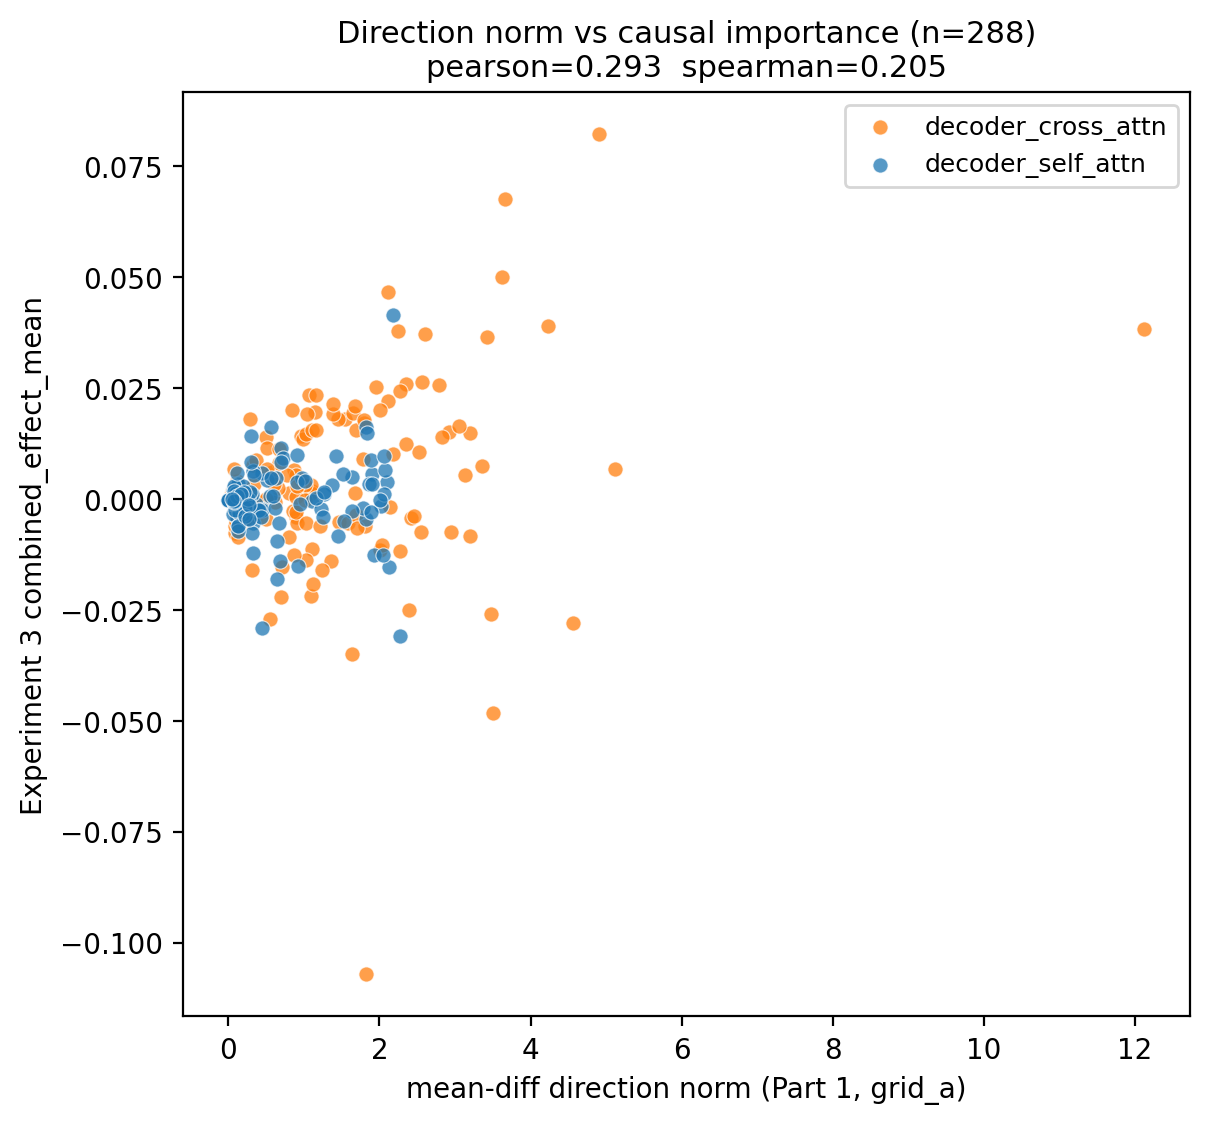
\includegraphics[width=0.72\textwidth]{outputs/plots/direction_norm_vs_exp3_effect.png}
  \caption{Per-head mean-diff direction norm (Part~1, grid\_a) vs.\
  Experiment~3's \texttt{combined\_effect\_mean} (causal importance), for
  all 288 decoder heads (144 \texttt{decoder\_self\_attn} + 144
  \texttt{decoder\_cross\_attn}). Pearson $r=0.293$, Spearman
  $\rho=0.205$.}
  \label{fig:normvseffect}
\end{figure}

\paragraph{Interpretation.} The correlation is positive but weak. This is a
genuine, interesting negative result: \textbf{the magnitude of a head's
linear mean-diff direction is only a modest predictor of its causal
importance.} The clearest counter-example is \texttt{L10-X-H0}, whose
direction norm ($12.13$) is nearly $3\times$ larger than the next-largest
head (\texttt{L9-X-H11}, $5.12$) and $\sim\!9\times$ the population mean
($1.41$), yet its Experiment~3 combined effect ($0.038$) is unremarkable
--- roughly the median of the flagged set --- and, as Section~\ref{sec:defense}
shows, its \emph{intervention} effect in this experiment is actually
consistently \emph{negative}. A large shift in the mean representation
between control and attack does not guarantee that shift is the
\emph{causally load-bearing} one; other, smaller-magnitude directions can
matter more for the actual score computation. Conversely the single
worst-correlated point, \texttt{L1-X-H7} (norm $1.82$, combined effect
$-0.107$, the most negative in the whole population), shows that a
mid-sized direction can also correspond to a head whose causal role is
\emph{opposed} to the attack, not aligned with it. Since Experiment~3 never
scored encoder heads, no equivalent correlation exists for
\texttt{encoder\_self\_attn} --- this is a structural fact, not a gap
(\texttt{DECISIONS.md}).

% =====================================================================
\section{Results: Part 2a --- Defense (Subtraction)}
\label{sec:defense}
% =====================================================================

\begin{figure}[H]
  \centering
  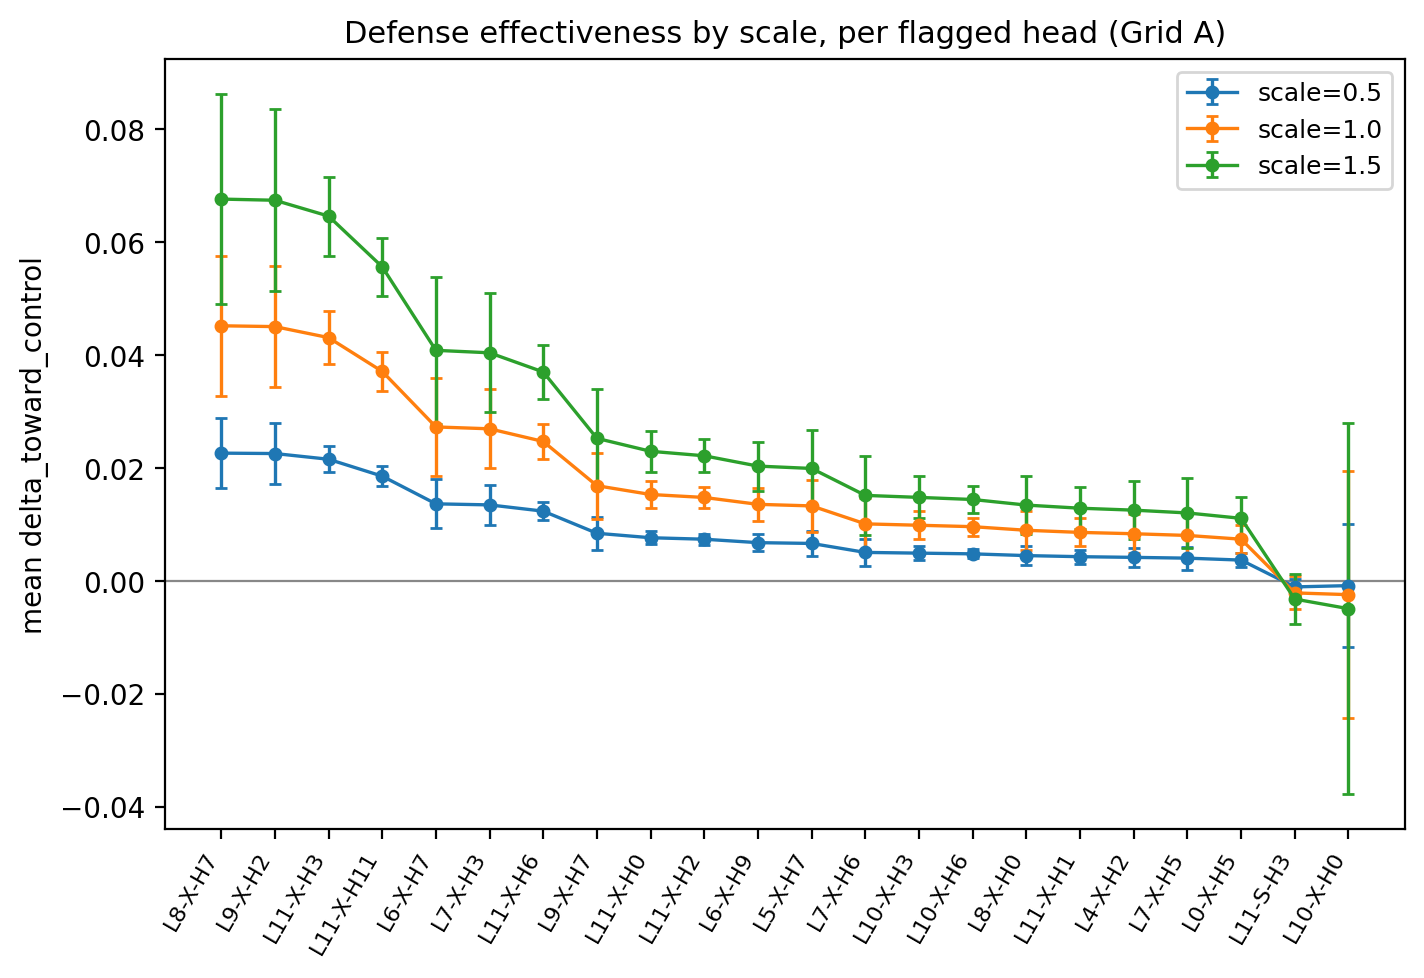
\includegraphics[width=0.95\textwidth]{outputs/plots/defense_by_scale_grid_a.png}
  \caption{Mean $\Delta_{\text{toward control}}$ (Eq.~\ref{eq:dtc}) per
  flagged head, one line per scale, pooled over all 105 attacks (grid\_a,
  $n{=}1050$ per point). Heads sorted descending by their scale-1.5 value.
  Error bars are $\pm 1$ std over the 1050 (attack, example) pairs.}
  \label{fig:defensebyscale}
\end{figure}

\begin{table}[H]
\centering
\caption{Top 10 flagged heads by defense effectiveness (grid\_a, best
scale, always $1.5$ except the two non-responding heads). $n{=}1050$ per
row.}
\label{tab:topdefense}
\begin{tabular}{lrrr}
\toprule
Head & Best scale & Mean $\dtc$ & Std $\dtc$ \\
\midrule
\texttt{L8-X-H7}  & 1.5 & 0.0677 & 0.0186 \\
\texttt{L9-X-H2}  & 1.5 & 0.0675 & 0.0161 \\
\texttt{L11-X-H3} & 1.5 & 0.0646 & 0.0070 \\
\texttt{L11-X-H11}& 1.5 & 0.0557 & 0.0052 \\
\texttt{L6-X-H7}  & 1.5 & 0.0409 & 0.0130 \\
\texttt{L7-X-H3}  & 1.5 & 0.0404 & 0.0105 \\
\texttt{L11-X-H6} & 1.5 & 0.0370 & 0.0047 \\
\texttt{L9-X-H7}  & 1.5 & 0.0253 & 0.0087 \\
\texttt{L11-X-H0} & 1.5 & 0.0230 & 0.0036 \\
\texttt{L11-X-H2} & 1.5 & 0.0222 & 0.0029 \\
\bottomrule
\end{tabular}
\end{table}

\paragraph{Interpretation.} \textbf{20 of the 22 flagged heads show a
monotonically increasing defensive effect with scale} --- for every one of
these heads, scale~$1.5$ beats scale~$1.0$ beats scale~$0.5$, and none of
the tested scales overshoots into negative territory (Eq.~\ref{eq:dtc}
never turns negative at any tested scale for these 20 heads). Since the
effect has not saturated by scale~$1.5$ (the largest tested), the natural
follow-up is whether even larger scales continue to help or eventually
overcorrect past the control baseline --- not tested here
(Section~\ref{sec:limits}). The two flagged heads that never help ---
\texttt{L10-X-H0} and \texttt{L11-S-H3} (the sole \texttt{decoder\_self\_attn}
head) --- are mildly \emph{harmful} at every scale, with the least-bad
(smallest-magnitude-harm) option being the smallest scale tested. Notably
\texttt{L10-X-H0} is exactly the head flagged above as having a
disproportionately large direction norm but weak/opposed causal role ---
consistent evidence, from two independent analyses, that this particular
head's mean-diff direction does not describe a useful intervention target.

\begin{figure}[H]
  \centering
  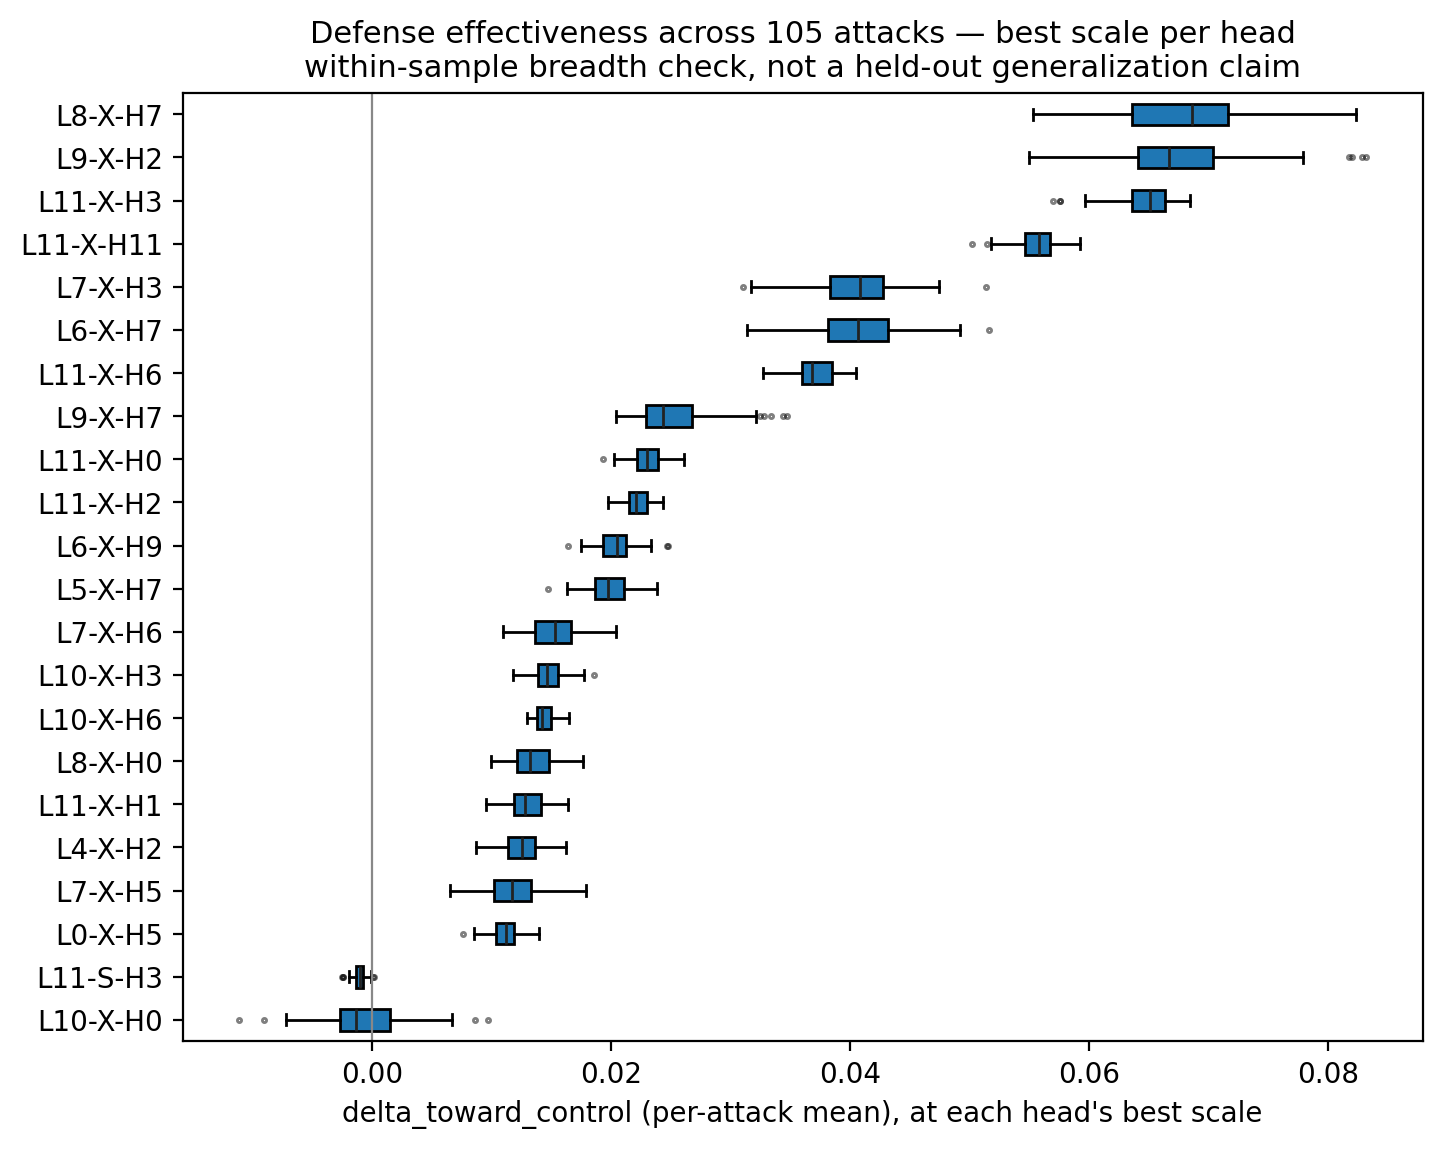
\includegraphics[width=0.8\textwidth]{outputs/plots/defense_across_attacks_best_scale_grid_a.png}
  \caption{Box plot of $\Delta_{\text{toward control}}$ across the 105
  attacks (one point per attack = that attack's mean over its 10 examples),
  at each head's own best scale. A tight box entirely above zero indicates
  the defense generalises consistently across attack types \emph{within
  this sample}; this is a breadth check, not a held-out claim.}
  \label{fig:defenseacross}
\end{figure}

\paragraph{Interpretation.} The breadth check (Figure~\ref{fig:defenseacross})
confirms the aggregate finding is not driven by a handful of attacks: for
the 20 responsive heads, the box for essentially every head sits clearly
above zero across the full spread of 105 attacks, with only mild
attack-to-attack variance (visible whiskers, few outlier points). The two
non-responsive heads (\texttt{L11-S-H3}, \texttt{L10-X-H0}) show boxes
straddling or below zero consistently, confirming their poor performance is
not an artefact of a specific subset of attacks.

\subsection{Grid B: does the attack-specific direction do better?}

\begin{table}[H]
\centering
\caption{Grid~A (pooled, generic direction) vs.\ Grid~B (single-attack
\texttt{relevant\_start\_5}, attack-specific direction) at each head's best
scale (always $1.5$). $n{=}1050$ for grid\_a, $n{=}100$ for grid\_b. Ratio
$>1$ means the attack-specific direction is a stronger defense on its own
attack than the generic pooled direction is, averaged across all attacks.}
\label{tab:gridab}
\begin{tabular}{lrrr}
\toprule
Head & Grid A $\dtc$ & Grid B $\dtc$ & Ratio (B/A) \\
\midrule
\texttt{L9-X-H2}  & 0.0675 & 0.2299 & 3.41 \\
\texttt{L11-X-H3} & 0.0646 & 0.1113 & 1.72 \\
\texttt{L8-X-H7}  & 0.0677 & 0.0984 & 1.45 \\
\texttt{L11-X-H11}& 0.0557 & 0.0879 & 1.58 \\
\texttt{L11-X-H6} & 0.0370 & 0.0724 & 1.95 \\
\texttt{L6-X-H7}  & 0.0409 & 0.0661 & 1.62 \\
\bottomrule
\end{tabular}
\end{table}

Across all 22 heads, the grid\_a and grid\_b best-scale defense scores
correlate at $r=0.879$ --- the same heads matter in both tiers, in almost
the same relative order --- but grid\_b's attack-specific direction is
\textbf{systematically 1.5--3.4$\times$ more effective} than grid\_a's
direction pooled across 105 attacks, evaluated on the one attack (\texttt{relevant\_start\_5})
both tiers share the most data for. This is the expected and reassuring
result: a direction fit specifically to one attack captures a sharper
signal than one averaged across 105 heterogeneous attacks (which include
weak and even score-\emph{decreasing} attacks, per Experiment~1's
cross-attack results), diluting the pooled direction. It also validates
that the two-tier design is doing meaningful work, not just duplicating
grid\_a at a different sample size.

% =====================================================================
\section{Results: Part 2b --- Sufficiency (Addition)}
% =====================================================================

\begin{figure}[H]
  \centering
  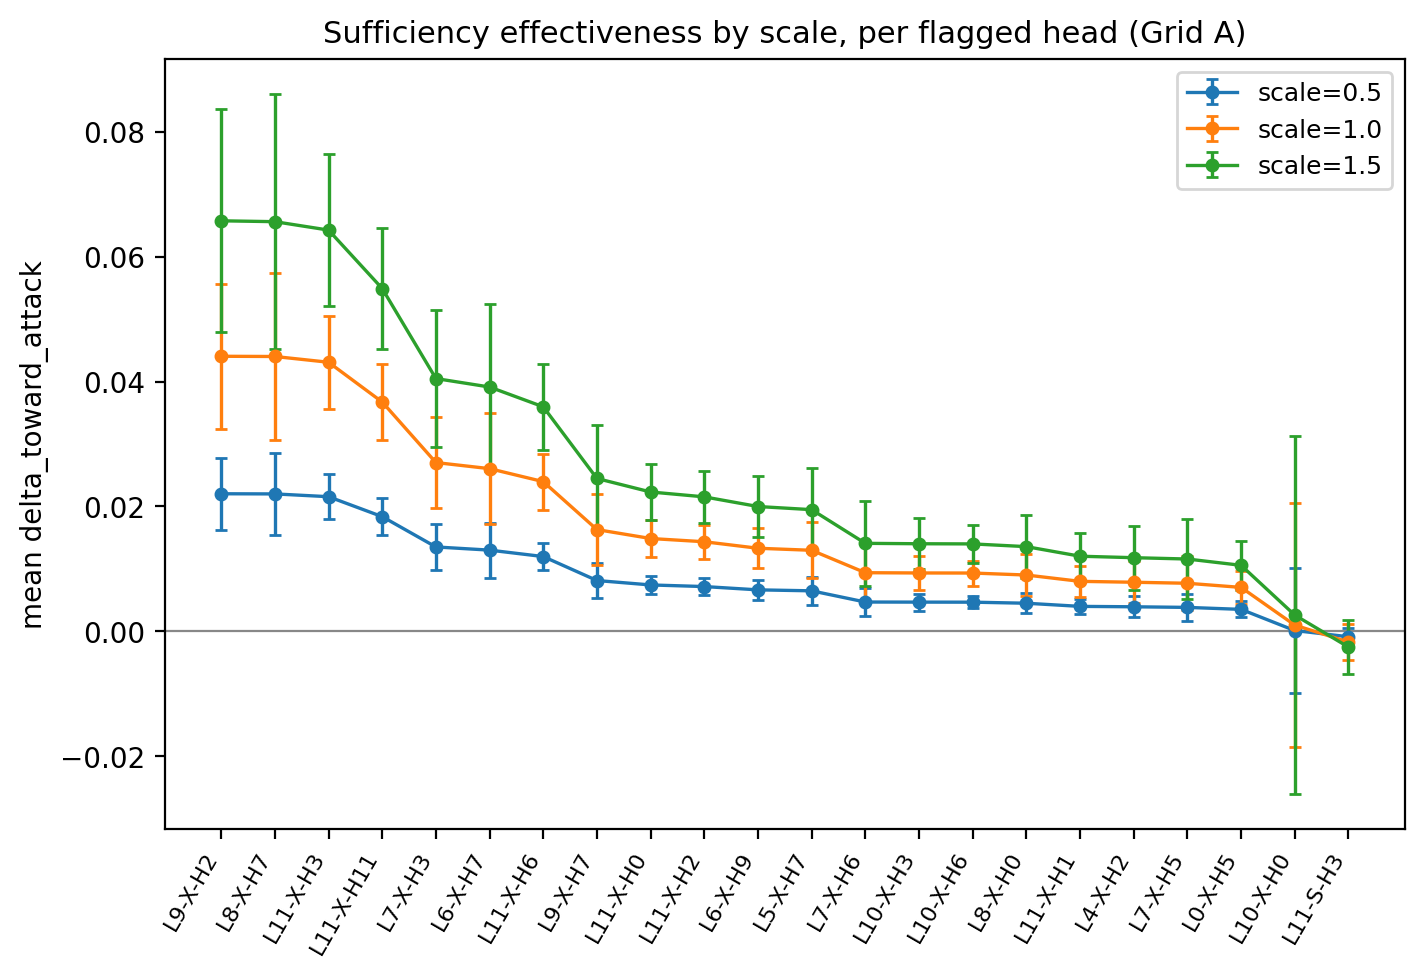
\includegraphics[width=0.95\textwidth]{outputs/plots/sufficiency_by_scale_grid_a.png}
  \caption{Mean $\Delta_{\text{toward attack}}$ (Eq.~\ref{eq:dta}) per
  flagged head, one line per scale, pooled over all 105 attacks
  (grid\_a, $n{=}1050$ per point).}
  \label{fig:sufficiencybyscale}
\end{figure}

\paragraph{Interpretation.} The sufficiency test (adding the direction to a
\emph{clean} input) produces an almost identical head ranking to the
defense test: the Pearson correlation between each head's best-scale
$\Delta_{\text{toward control}}$ and $\Delta_{\text{toward attack}}$ across
all 22 heads is $r=0.999$, and the same two heads
(\texttt{L10-X-H0}, \texttt{L11-S-H3}) are again the only non-responders.
This is strong evidence that the direction is genuinely
\textbf{bidirectional}: it is not merely that subtracting \emph{something}
from an attacked activation happens to help (which could be true even for
an arbitrary or noisy vector, simply by reducing activation magnitude) ---
the \emph{same} vector, added the other way, is independently sufficient to
push a clean input's score toward attack-like values. The magnitudes are
close but not identical (e.g.\ \texttt{L9-X-H2}: $\dtc=0.0675$ vs.\
$\dta=0.0658$ in grid\_a; grid\_b shows the same pattern, e.g.\
\texttt{L9-X-H2}: $0.2299$ vs.\ $0.2223$), consistent with the score
function being a smooth but not perfectly linear function of the head's
activation around the clean/attack operating points.

% =====================================================================
\section{Overall Interpretation and Discussion}
% =====================================================================

\begin{enumerate}
  \item \textbf{A simple linear direction is a real, usable defense signal
        at most flagged heads.} 20 of the 22 heads Experiment~3 identified
        as causally important also yield a mean-diff direction whose
        subtraction reliably moves the attacked score back toward the
        clean baseline, with the effect growing (not saturating) up to the
        largest tested scale ($1.5\times$). This is a substantially cheaper
        intervention than activation patching, since it requires no second
        forward pass over a donor input at inference time --- only a fixed,
        precomputed vector.
  \item \textbf{The direction is bidirectional, not a one-way trick.} The
        near-perfect ($r{=}0.999$) agreement between the defense (subtract)
        and sufficiency (add) head rankings shows the direction captures a
        genuine, consistent axis of the attack's effect on each head's
        representation, not an artefact of one particular intervention
        sign.
  \item \textbf{Direction magnitude is a weak, sometimes misleading, proxy
        for causal importance.} The single largest-norm head in the entire
        decoder (\texttt{L10-X-H0}) is one of only two flagged heads whose
        intervention never helps. Selecting intervention targets by
        \texttt{combined\_effect} (Experiment~3's causal metric) rather
        than by raw direction norm is clearly the right choice, and this
        experiment provides direct evidence for why.
  \item \textbf{Attack-specific directions are stronger than pooled ones.}
        The grid\_b (single-attack) direction is 1.5--3.4$\times$ more
        effective than the grid\_a (105-attack pooled) direction on the
        attack both tiers share, while preserving almost the same head
        ranking ($r{=}0.879$). A production defense would likely want to
        either fit per-attack-family directions or accept a diluted,
        pooled direction as the price of generality.
\end{enumerate}

% =====================================================================
\section{Limitations and Threats to Validity}
\label{sec:limits}
% =====================================================================

\begin{itemize}
  \item \textbf{In-sample only.} The direction is fit and tested on the
        \emph{same} example pool per tier. This establishes feasibility ---
        a mean-diff direction \emph{can} work as a defense on the examples
        it was computed from --- but says nothing about whether the same
        direction generalises to held-out examples or held-out attacks.
        This is a deliberate scope limitation stated in the original task
        and \texttt{DECISIONS.md}, not an oversight, but any claim of a
        practical defense would need a held-out evaluation.
  \item \textbf{Scale range not saturated.} All 20 responsive heads are
        still improving at the largest tested scale ($1.5$); the point of
        diminishing or negative returns (overcorrection past the control
        baseline) was not found.
  \item \textbf{Single-head interventions only.} Every intervention shifts
        exactly one head; joint/multi-head shifts (which could interact
        non-additively) were not tested.
  \item \textbf{Encoder heads never intervened on.} Part~1 computes
        \texttt{encoder\_self\_attn} directions descriptively, but Part~2
        never tests them, since Experiment~3's flagged list --- the sole
        source of Part~2's scope --- contains no encoder heads by
        construction (encoder was out of scope for Experiment~3).
  \item \textbf{Sample size.} Grid~A uses only 10 examples per attack (1050
        total); Grid~B's 100-example canonical-attack tier is more stable
        but covers only one attack.
\end{itemize}

% =====================================================================
\section{Reproducibility}
% =====================================================================

From the experiment directory, with the \texttt{advseq2seq} conda
environment:

\begin{lstlisting}
python scripts/00_derive_flagged_heads.py --config configs/default.yaml
python scripts/01_compute_directions.py   --config configs/default.yaml  # Part 1
python scripts/02_run_interventions.py    --config configs/default.yaml  # Part 2
python scripts/03_aggregate.py            --config configs/default.yaml
python scripts/04_make_plots.py           --config configs/default.yaml
# or, equivalently:
bash bash/run_all.sh configs/default.yaml
\end{lstlisting}

\noindent Both scripts~01 and~02 are resume-safe via per-tier / per-(tier,
attack) \texttt{status.json} files, following the same convention as
Experiments~1 and~3. A CPU-only smoke config
(\texttt{configs/smoke.yaml}) and a 12-test \texttt{pytest} suite
(hook correctness, direction arithmetic, additive-shift no-op-at-zero-scale,
metric formulas) verify the pipeline before a full SLURM run.

% =====================================================================
\section*{Appendix: Glossary of Key Quantities}
\addcontentsline{toc}{section}{Appendix: Glossary of Key Quantities}
% =====================================================================

\begin{description}[leftmargin=1.6em,style=nextline]
  \item[$\score$] $\operatorname{logit}(\texttt{true})-\operatorname{logit}(\texttt{false})$ at the first decoder step.
  \item[$\dirvec$] mean-diff direction, Eq.~\eqref{eq:direction}: mean(attack) $-$ mean(control) activation.
  \item[$\dtc$] Eq.~\eqref{eq:dtc} --- did subtracting $\dirvec$ from the attacked activation move the score toward control?
  \item[$\dta$] Eq.~\eqref{eq:dta} --- did adding $\dirvec$ to the clean activation move the score toward attack?
  \item[grid\_a / grid\_b] breadth (105 attacks, pooled direction) / depth (\texttt{relevant\_start\_5} only, attack-specific direction) tiers.
  \item[flagged heads] the 22 heads with Experiment~3 \texttt{combined\_effect\_mean} $> 0.02$.
  \item[whole-vector / per-head] direction granularity: full 768-dim sub-layer output, or one head's 64-dim slice.
\end{description}

\end{document}
